\documentclass{article}

\usepackage[T1]{fontenc}
\usepackage{mathptmx}
\usepackage{setspace}
\usepackage[top=1in,bottom=1in,left=3cm,right=2.4cm]{geometry}
\usepackage{listings}
\usepackage{graphicx}
\usepackage{subcaption}
\usepackage[sort&compress]{natbib}
\usepackage{hyperref}
\hypersetup{
	colorlinks,
	linkcolor=red,
	urlcolor=blue
}
\urlstyle{same}


\begin{document}
	\title{M1 Projet Long : Intermediate Report} 
	\author{Bey Nesrine, Gresh Clément}
	
	\date{Université de Paris - 2021-2022 }
	
	\maketitle
	


	
	\section{ Presentation }\label{sec:first}
	We wanted to develop an application that could actually be useful (even though we acknowledge it might not be finished by the end of the school year). That is why the two possible projects that we had in mind were :

\begin{enumerate}
  \item a program able to send to a list of students mathematical or programming exercises that could be corrected automatically.
  \item a program able to identify signs from the French Sign Language (LSF) through a video stream and translate them into text. It could then easily be read outloud by a device such as a smartphone or a computer.
\end{enumerate}

In the end, we decided for the latter because of our shared interest in image recognition. Even though we have never worked on that subject, it seemed like a more original and challenging topic. We decided to write the code in Pyhton as it is a widespread programming language that we were both unfamiliar with. This project is split into two main parts: 
\begin{enumerate}
  \item detecting and isolating a hand on a video stream, as well as finding the coordinates of its different landmarks (such as the phalanges).
  \item recognizing signs from the LSF using those data, from the most basic ones to the ones that use motion or have to take into account other body parts (e.g. the face).
\end{enumerate}

Thanks to \textbf{OpenCV} and \href{https://mediapipe.dev/}{\textbf{MediaPipe}}, it is pretty straightforward to identify the different landmarks of a hand and get their coordinates. This ensures that we can work on the second part while the first one is still in development.
	

	\begin{figure}[h!]
		\center
		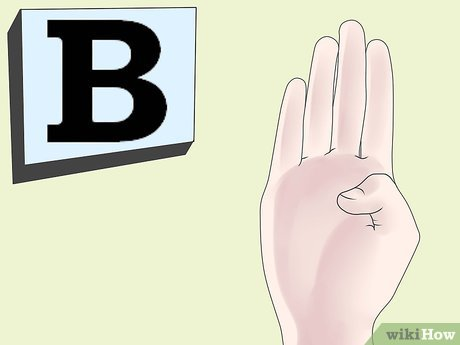
\includegraphics[width=70mm]{lettre-B.jpg}
		\caption{Letter B in the French Sign Language}
	\end{figure}



	\newpage\section{ Progress }\label{sec:second}
	As previously explained, we decided to work on two different branches : the first one aims to identify a hand and its landmarks on a video stream. The second one focuses on recognizing signs of the LSF.

In both cases, the main function allows to capture a video stream from a camera and show it on the screen after it was processed, displaying, for instance, the FPS or the position of the hand that was detected. The application stops when the "q" key is hit.

	\subsection{Hand tracking}\label{sec:first}
On the branch "HandTracking", the goal is to reproduce the MediaPipe functionalities used in the "SignRecognition" branch in order to detect a hand and find the coordinates of its landmarks. The steps that have been implemented so far thanks to OpenCV are :
\begin{enumerate}
  \item converting the input video stream from BGR (the default for OpenCV) to either RGB or Grayscale depending on the needs of the application.
  \item removing the parts of the image that don't match the potential color of a hand. For now, this is done using color ranges but will be improved using machine learning and databases of hand skin colors (see part 4).
  \item finding the contours of the remaining objects on the image. Several OpenCV methods are used here to blur the image, find the edges on it, dilate them and finally display them.
\end{enumerate}


	\subsection{Sign recognition}\label{sec:first}
Using MediaPipe functionalities, the program can currently determine very precisely the position of the hand as well as a specific fingertip's coordinates. These data are then used to determine information that are useful for sign recognition. For instance, the relative positions of the phalanges of a finger can help determine whether the finger is in flexion or extension.

To be more precise, when the frames are captured on camera, the methods in the "HandTracker" module allow to identify the landmarks of the hand(s) that are then stored in a list with the number of each landmark, along with their coordinates. All of this is possible thanks to an intensive use of the MediaPipe module. By using this information, we can determine and compare the positioning of each one of the points and therefore know which sign is made in front of the camera.

Therefore, the program can now recognize a set of simple letters of the \textbf{Sign Language Alphabet}: A, B, E, F and U.

	\begin{figure}[h!]
		\center
		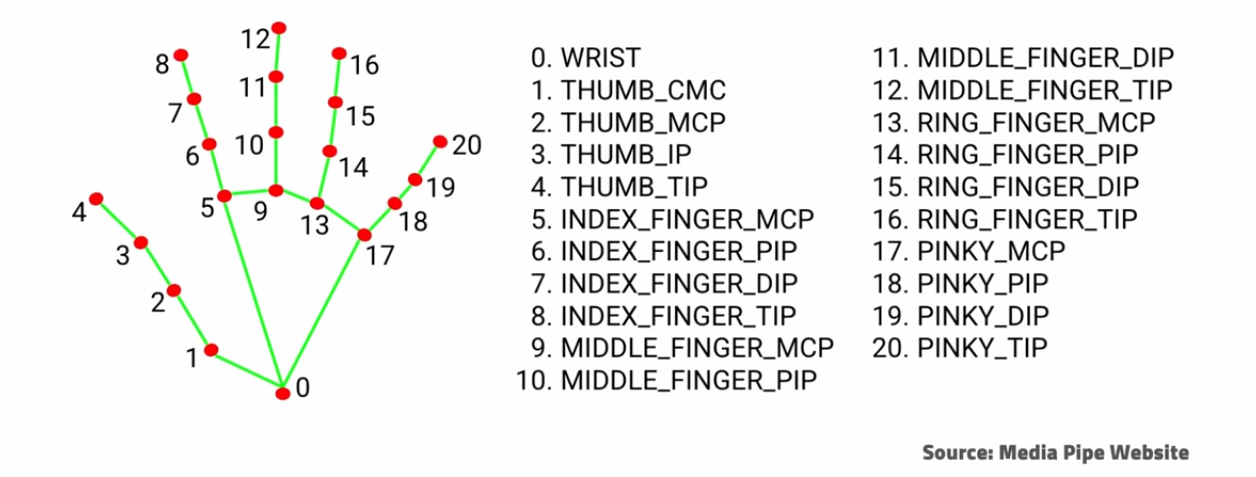
\includegraphics[width=\linewidth]{landmarks.png}
		\caption{ hand landmarks}
	\end{figure}


	\newpage

	
	\section{Difficulties}\label{sec:third}
	The MediaPipe module greatly helped in the development of this project, but reproducing its functionality of detecting a hand is proving tricky (as expected).  It is especially challenging because, although the shape or edges can be correctly identified, it remains difficult to determine where the landmarks are.

	We are also having trouble finding databases that match our needs for the machine learning part of the project (see part 4). In particular, one for the French \textbf{Sign Language Alphabet}.

	Finally, we are unsure how to take into account motion in our algorithm, which is required for some signs like J, P or Z.
	
	\section{Next Steps}\label{sec:fourth}
	
	Wether it is to recognize a hand on a video stream or the sign formed by said hand, our next step is to use unsupervised machine learning algorithms, such as the \textbf{k-means} algorithm, in order to form clusters of data and automate part of the detection. Doing so will require finding proper image banks and identifying criteria that will be used for the detection, such as the color of the hand (for hand recognition) or the position of each phalanx compared to the others (for sign recognition). This should also allow to greatly improve the precision of the algorithm.
	
	Regarding the hand tracking branch, the next step is to pinpoint some landmarks (fingers or phalanges). While on the sign recognition branch, it is to identify more complex signs, such as the ones that require face recognition, body gestures and movements. 
	
	
	
\end{document}

